%%%%%%%%%%%%%%%%%%%%%%%%%%%%%%%%%%%%%%%%%%%%%%%%%%%%%%%%%%%%%%%%%%%%%%%%%%%%%%%%%%%%%%%%%%%%%%%%%%%%%%%%%%%%%%%%%%%%%%%%%%%%%%%%%%%%%%%%%%%%%%%%%%%%%%%%%%%
% This is just an example/guide for you to refer to when submitting manuscripts to Frontiers, it is not mandatory to use Frontiers .cls files nor frontiers.tex  %
% This will only generate the Manuscript, the final article will be typeset by Frontiers after acceptance.                                                 %
%                                                                                                                                                         %
% When submitting your files, remember to upload this *tex file, the pdf generated with it, the *bib file (if bibliography is not within the *tex) and all the figures.
%%%%%%%%%%%%%%%%%%%%%%%%%%%%%%%%%%%%%%%%%%%%%%%%%%%%%%%%%%%%%%%%%%%%%%%%%%%%%%%%%%%%%%%%%%%%%%%%%%%%%%%%%%%%%%%%%%%%%%%%%%%%%%%%%%%%%%%%%%%%%%%%%%%%%%%%%%%

%%% Version 3.1 Generated 2015/22/05 %%%
%%% You will need to have the following packages installed: datetime, fmtcount, etoolbox, fcprefix, which are normally inlcuded in WinEdt. %%%
%%% In http://www.ctan.org/ you can find the packages and how to install them, if necessary. %%%

\documentclass{frontiersSCNS} % for Science, Engineering and Humanities and Social Sciences articles
%\documentclass{frontiersHLTH} % for Health articles
%\documentclass{frontiersFPHY} % for Physics and Applied Mathematics and Statistics articles

%\setcitestyle{square}
\usepackage{url,hyperref,lineno,microtype}
%\usepackage{titlesec}
\usepackage[onehalfspacing]{setspace}
%\linenumbers
%\setcounter{secnumdepth}{4}

% Leave a blank line between paragraphs instead of using \\


\def\keyFont{\fontsize{8}{11}\helveticabold }
\def\firstAuthorLast{Clark {et~al.}} %use et al only if is more than 1 author
\def\Authors{Daniel Clark\,$^{1}$, Steven Giavasis\,$^{1}$, Christian Haselgrove\,$^{2}$, David N. Kennedy\,$^{2}$, Zhizhong Liu\,$^{3}$, Michael Milham\,$^{1,4}$, Petros Petrosyan\,$^{3}$, Carinna M. Torgerson\,$^{3}$, John D. Van Horn\,$^{3}$ and R. Cameron Craddock\,$^{1,5,*}$}
% Affiliations should be keyed to the author's name with superscript numbers and be listed as follows: Laboratory, Institute, Department, Organization, City, State abbreviation (USA, Canada, Australia), and Country (without detailed address information such as city zip codes or street names).
% If one of the authors has a change of address, list the new address below the correspondence details using a superscript symbol and use the same symbol to indicate the author in the author list.
\def\Address{$^{1}$Center for the Developing Brain, Child Mind Institute, New York, NY, USA\\
$^{2}$Division of Informatics, Department of Psychiatry, University of Massachusetts Medical School, Worcester, MA, USA\\
$^{3}$The Institute for Neuroimaging and Informatics (INI) and Laboratory of Neuro Imaging (LONI), Keck School of Medicine of USC, University of Southern California, Los Angeles, CA, USA\\
$^{4}$Center for Biomedical Imaging and Neuromodulation, Nathan S. Kline Institute for Psychiatric Research, Orangeburg, New York, USA\\
$^{5}$Computational Neuroimaging Laboratory, Center for Biomedical Imaging and Neuromodulation, Nathan S. Kline Insitute for Psychiatric Research, Orangeburg, NY, USA}
% The Corresponding Author should be marked with an asterisk
% Provide the exact contact address (this time including street name and city zip code) and email of the corresponding author
\def\corrAuthor{R. Cameron Craddock}
\def\corrAddress{Computational Neuroimaging Laboratory, Center for Biomedical Imaging and Neuromodulation, Nathan S. Kline Insitute for Psychiatric Research, Orangeburg, NY, 10962, USA}
\def\corrEmail{email@uni.edu}


\begin{document}
\onecolumn
\firstpage{1}

\title[Harnessing cloud computing]{Harnessing cloud computing for high capacity analysis of neuroimaging data} 

\author[\firstAuthorLast ]{\Authors} %This field will be automatically populated
\address{} %This field will be automatically populated
\correspondance{} %This field will be automatically populated

\extraAuth{}% If there are more than 1 corresponding author, comment this line and uncomment the next one.
%\extraAuth{corresponding Author2 \\ Laboratory X2, Institute X2, Department X2, Organization X2, Street X2, City X2 , State XX2 (only USA, Canada and Australia), Zip Code2, X2 Country X2, email2@uni2.edu}


\maketitle

%%%%%%%%%%%%%%%%%%%%%%%%%%%%%%%%%%%%%%%%%%%%%%%%%%%%%%%%%%%%%%%%%%%%%%%%%%%%%%%%%%%%%%%%%%%%%%%%%%%%%%%%%%%%%%%%%%%%%%%%%%%%%%%%%%%%%%%%%%%%%%%%%%%%%%%%%%%%%%%%%%%%%%%%%%%%%%%%%%%%%%%%%%%%%%%%%%%%%%%%%%%%%%%%%%%%%%%%%%%%%%%%%%%%%%%
%%% The sections below are for reference only.
%%%
%%% For Original Research Articles, Clinical Trial Articles, and Technology Reports the section headings should be those appropriate for your field and the research itself. It is recommended to organize your manuscript in the
%%% following sections or their equivalents for your field:
%%% Abstract, Introduction, Material and Methods, Results, and Discussion.
%%% Please note that the Material and Methods section can be placed in any of the following ways: before Results, before Discussion or after Discussion.
%%%
%%%For information about Clinical Trial Registration, please go to http://www.frontiersin.org/about/AuthorGuidelines#ClinicalTrialRegistration
%%%
%%% For Clinical Case Studies the following sections are mandatory: Abstract, Introduction, Background, Discussion, and Concluding Remarks.
%%%
%%% For all other article types there are no mandatory sections.
%%%%%%%%%%%%%%%%%%%%%%%%%%%%%%%%%%%%%%%%%%%%%%%%%%%%%%%%%%%%%%%%%%%%%%%%%%%%%%%%%%%%%%%%%%%%%%%%%%%%%%%%%%%%%%%%%%%%%%%%%%%%%%%%%%%%%%%%%%%%%%%%%%%%%%%%%%%%%%%%%%%%%%%%%%%%%%%%%%%%%%%%%%%%%%%%%%%%%%%%%%%%%%%%%%%%%%%%%%%%%%%%%%%%%%%

% Abstract
\begin{abstract}
%%% Leave the Abstract empty if your article falls under any of the following categories: Editorial Book Review, Commentary, Field Grand Challenge, Opinion or specialty Grand Challenge.
\section{}
%As a primary goal, the abstract should render the general significance and conceptual advance of the work clearly accessible to a broad readership. References should not be cited in the abstract.
For full guidelines regarding your manuscript please refer to \href{http://www.frontiersin.org/about/AuthorGuidelines}{Author Guidelines} \\ or \textbf{Table \ref{Tab:01}} for a summary according to article type.

\tiny
 \keyFont{ \section{Keywords:} Cloud computing, high-performance compute clusters, neuroimaging preprocessing, AWS, spot instances } %All article types: you may provide up to 8 keywords; at least 5 are mandatory.
\end{abstract}

% Introduction
\section{Introduction}

intro

% Methods
\section{Methods}

%% AWS EC2
\subsection{The Amazon Web Services Elastic Compute Cloud}

Amazon provides a collection of remote computing services called Amazon Web Services (AWS). One of the most fundamental and well-known of these services is Amazon Elastic Compute Cloud (EC2). EC2 allows for the configuration and use of virtual servers, or compute instances, at any capacity desired. In contrast with the up-front research and costs necessary to purchase an in-house computing solution, EC2 offers the flexibility to utilize a wide range of computing capacity with a "pay-as-you-go" model. The associated costs are divided between processing/compute hours, storage amount, and data transfer/networking traffic. AWS is offered across multiple regions hosted at different data centers spread out over the world with each region subdivided into “availability zones”. For example the “us-east-1” region is centered in northern Virginia and its services are subdivided among the “us-east-1a”, “us-east-1b”, “us-east-1c”, and “us-east-1e” availability zones. This framework makes it possible to optimize one's computing power, budget, and locality for their application.

%%% Instances and AMIs
\subsubsection{Instances and AMIs}

EC2 offers ``instances" which represent the hardware resources that will perform computation.  To deliver consistent performance, the hardware underlying instances are bundled by Amazon into virtual processors, called Amazon EC2 Compute Units (ECUs). ECUs are routinely benchmarked and tested to ensure stability even as hardware is modified or updated. A range of ``instance types" are available to support a variety of different use cases. Instance types include ``general purpose" instances (e.g. t2.micro, t2.small, m4.xlarge), with low to moderate computing power, ``compute optimized" instances (e.g. c3.large, c3.8xlarge, c4.4xlarge) that have a higher quantity of CPUs, ``memory optimized" instances (e.g. m3.2xlarge, r3.xlarge, r3.8xlarge) containing large amounts of RAM, ``storage optimized" instances (e.g. i2.xlarge, i2.4xlarge, d2.8xlarge) for high data I/O throughput and capacity, and GPU instances (e.g. g2.2xlarge, g2.8xlarge). As of June 2015, the ``compute optimized" instances run with Intel Xeon E5-2666 v3 (Haswell) processors.


The software ecosystem to be run on an instance is provided by an Amazon Machine Image (AMI). AMIs are analogous to virtual machine images and contain the operating system, software, and data for a virtual server. Users can choose from thousands of preconfigured AMIs from the AWS and community marketplaces or can create their own. AMIs are available using Linux or Windows operating systems and are priced for hourly or yearly usage; many Linux-based AMIs are free.


Preconfigured AMIs provide users with a platform-as-a-service in which they rely on the developer to configure and maintain the software ecosystem. This allows developers to focus on maintaining one central system that can be deployed as needed, rather than keeping multiple resources up-to-date. This solution is novel as it allows for centralized system administration with dynamically-sized ``elastic" computing resources; end-users only pay for what they use and without having to perform configuration or maintenance themselves.

%%%% On-demand instances
\paragraph{On-demand instances}

One of the ways to pay for and use EC2 instances is via on-demand pricing. In this schema, the user can request their desired resources at any time by paying the on-demand hourly rates. The instances are available to them immediately without interruptions and will continue to be active until explicitly terminated. The cost of on-demand instances is significantly higher than other purchasing mediums, but is useful for time-sensitive tasks.

%%%% Reserved instances
\paragraph{Reserved instances}

Another payment system is to use reserved instances. If there is long term interest in using EC2 and demand for resources is pretty consistent over time, users can pay up-front, or throughout the reservation duration (1 year or 3 years) to reserve instances to be used at any time. The cost is reduced resulting in savings of up to 75\% compared with on-demand instances.

%%%% Spot instances
\paragraph{Spot instances}

Amazon allows for users to bid on the resources that are not being used at a significant discount, up to 90\%, compared to on-demand pricing. The instances themselves operate in the exact same way as an on-demand or reserved instance would; the major difference with spot is the chance of forced termination if the spot price equals or exceeds the user bid price. With spot pricing, the hourly cost for an instance can vary depending on market demand. This provides great flexibility for cost and computing demands as long as the type of processing can handle sudden interruptions and recover.

% EC2 instnace pricing table
\begin{table}[!t]
%\textbf{\refstepcounter{table}\label{Tab:01} Table \arabic{table}.}{ Instance types pricing}

\processtable{ Instance types pricing}
{\begin{tabular}{lllllll}\toprule
    Instance type & vCPUs & ECUs & Memory (GiB) & On-demand (\$/hr) & Reserved no-upfront, 1 year (\$/hr) & Typical spot (\$/hr)\\\midrule
    t2.small & 1 & Variable & 2 & 0.026 & 0.018 & N/A\\
    m3.xlarge & 4 & 13 & 15 & 0.266 & 0.190 & 0.0334\\
    c3.8xlarge & 32 & 108 & 60 & 1.680 & 1.168 & 0.350\\
    g2.2xlarge & 8 & 26 & 15 & 0.650 & 0.474 & 0.075
\end{tabular}}{*All prices reflect the us-east-1 northern Virginia region}
\end{table}

%%% Data storage
\subsubsection{Data storage}

%%%% EBS
\paragraph{Elastic block storage}
Data storage pricing is offered for two storage mediums in EC2: elastic block storage (EBS) and instance storage. EBS offers block-level storage volumes that can be treated like disk drives that support formatting of file systems (such as NFS or NTFS). These volumes can be attached to running instances and persist even after the instance is shut down or terminated. EBS volumes are billed based on GB-months of storage, IOPS, and I/O requests, depending on the type of EBS storage used.

%%%% Instance storage
\paragraph{Instance storage}
Instance storage is also a block-level storage medium available in EC2, however, it is only available with certain instance types, at certain sizes, and only persists as long as the instance is up and running. Instance storage is located on disks that are physically attached to the host instance and will lose all data when the instance is stopped or terminated. The pricing for instance storage is built into the hourly price of using the associated instance - this makes it a cheaper option than EBS if data need only persist as long as the instances. Instance storage also provides for optimizing storage costs by keeping unnecessary or temporary files with the instance, and storing valuable files on smaller EBS volumes.

%%%% S3
\paragraph{S3}
Amazon also offers their Simple Storage Service (S3) platform as a cost efficient and robust alternative to solutions in EC2. S3 uses object-level storage in user-defined “buckets”, rather than block-level storage and can be accessed from anywhere via their web interface or API. S3 storage comes in standard, reduced redundancy, and glacier storage costs - depending on the importance or access time needed of the data. Standard storage offers the most readily accessible and robust data with 99.999999999\% durability, where reduced redundancy offers slightly less robustness with 99.99\% durability, but at a reduced cost. Glacier is Amazon’s data archiving service that allows users to store backups of their S3 data at a further reduced cost, with the tradeoff of waiting 3 to 5 hours to access the data again.


All storage services prices are based on per-GB of data at various tiers of overall storage being utilized in S3 (e.g. \$0.03 per GB for up to 1TB of overall storage per month); these prices vary between regions. Additional costs are associated with the amount of requests (e.g. PUT, DELETE, COPY, LIST) made on the S3 objects. However, the costs are much lower compared with long-term data storage in EC2.

%%% Data transfer
\subsubsection{Data transfer}
There are costs associated with the amount of data transferred in and out of AWS. Data transfer in to EC2 from anywhere on the internet is completely free for all regions. However, there are costs associated with transferring data out to the internet (priced per GB), depending on how much data in total is transferred monthly. Data transfer is free between instances in EC2 as long as they are in the same availability zone and use private IP addresses.


Data transfer pricing has a fairly simple structure in S3. It is free to upload data to S3 from anywhere. Costs are associated for every GB of data downloaded from S3 to the internet in a similar monthly total tier that EC2 uses. However, downloading data from S3 is free to EC2 instances in the same AWS region as the S3 bucket of interest.

%%% Databases
\subsubsection{Databases}
Amazon offers a variety of database solutions in AWS, each of which are tailored for specific use cases. For relational databases, Amazon Relational Database Service (RDS) provides a range of database engines, including MySQL, Oracle, PostgreSQL, and more. RDS abstracts away the administrative overhead with setting up a database and provides automatic backups and elastic compute resources using their API.


Other solutions include DynamoDB, for NoSQL databases with a lower and more predictable workload, Elasticache, for in-memory cache rapid access of data, and Redshift, for high-performance big-data warehousing. Additionally, users can host their choice of database engine, with any configuration, on EC2 instances.

%%% Data privacy, security, and HIPAA
\subsubsection{Data privacy, security, and HIPAA}
Amazon has built a robust security infrastructure around their web services, with many features being specifically targeted for regulatory compliance. Security administration in AWS is mostly the same as it is with in-house servers, with security patches, backups, anti-virus software, user permissions, ACLs, traffic monitoring, and data encryption. Hardware VPNs can be set up between local and cloud resources as well.
There are a few administrative differences with regard to security, as the resources are being managed by the user remotely. These include utilizing software-based security instead of hardware-based approaches, issuing user credential keys for access, configuring private networks using AWS Virtual Private Cloud (VPC), setting up firewalls around each EC2 instance in the form of security groups, and dealing with geographical isolation between regions. It is important to note that security is now a shared responsibility between the user and AWS. The security associated with hardware, networking, facilities, and infrastructure software is managed by Amazon. The robustness and security of these are top priority and are routinely audited by third parties for compliance. The user is responsible for who has access to their resources, software security patches, data encryption, network firewalls, and backup and archiving preferences; overall the user is responsible for the proper configuration of the AWS infrastructure to keep data secure and private. This relationship is outlined in detail in the ``AWS Shared Responsibility Model."


Utilizing AWS resources to process and store PHI data requires HIPAA and HITECH compliance; as such, any institutions dealing with PHI needs to be HIPAA-certified. HIPAA certification is not specifically available for cloud computing providers like AWS. However, AWS has aligned their risk management program with FedRAMP and NIST 800-53 security standards; NIST (the National Institute of Standards and Technology) has supported this as a valid approach for satisfying the HIPAA security rule, which states ``the EPHI that a covered entity creates, receives, maintains, or transmits must be protected against reasonably anticipated threats, hazards, and impermissible uses and/or disclosures." This allows for any HIPAA-certified institution to use AWS services for the processing, transmission, and storage of PHI data, as long as they take the proper precautions.


HIPAA rules require covered institutions enter into a contract with any non-covered subcontractors or businesses to guarantee both are aware and take precautions to guard the integrity of PHI; this contract is known as a ``Business Associate Agreement" (BAA). Amazon offers a standard BAA and will sign with HIPAA-covered institutions, given that both parties obey the AWS Shared Responsibility Model.


Once the user has signed a BAA with Amazon, all AWS services are available to them, but only six services should be used when dealing with PHI: Amazon EC2, Amazon EBS, Amazon S3, Amazon Redshift, Amazon Glacier, and Amazon Elastic Load Balancer. AWS has set up each of these services to provide for any and all HIPAA safeguards in their configurations; the default configurations on any of these services are typically the most stringent and secure. The responsibilities fall to the user to ensure proper user access and permissions, which can be controlled with AWS Identity and Access Management (IAM) service, firewalls, and traffic restrictions to specific IP ranges. System administrators interacting with AWS can grant users access with key or token credentials. Additionally, PHI data should always be encrypted before, during, and after transfer to AWS in accordance with HIPAA regulations; this can be achieved using technologies such as 256-bit AES encryption algorithms. Finally, HIPAA requires robust data-backup and disaster-recovery procedures as well as the ability to audit systems for their security and PHI data provenance. AWS offers the ability to chronologically snapshot any EBS volumes in EC2 and back up all relevant data to S3, where it is copied across data centers and securely stored. Additionally, AWS employees are not able to log into customer instances in EC2 and S3 data access is highly restricted. In the end, the easiest way to ensure HIPAA-compliance is to always use anonymized data and avoid the upload of PHI information.


Currently other HIPAA-covered entities are using the AWS infrastructure for their health care services and many HIPAA compliance case studies can be found on the AWS website.

%% Neuroimaging in the cloud
\subsection{Neuroimaging in the cloud}

%%% AMIs and software tools
\subsubsection{AMIs and software tools}
AWS allows researchers in neuroimaging to process and analyze their data using the aforementioned computational and storage resources. Several organizations and laboratories have developed AMIs in EC2 as a platform-as-a-service to offer neuroimaging pipelines to the general public. These include the Configurable-Pipeline for the Analysis of Connectomes (C-PAC), the Neuroimaging Informatics Tools and Resources Clearinghouse (NITRC) Computational Environment (CE), Human Connectome Project (HCP), and the Laboratory of Neuro Imaging (LONI) AMIs. All of these are available either on the AWS or community marketplaces in EC2 for free use. Each AMI comes with the necessary software dependencies and system configuration to make neuroimaging analysis ready out-of-box and straightforward. The Debian-based AMIs use NeuroDebian as a software repository resource for neuroscience software; this makes installing and updating many common packages, like AFNI and FSL, easy for anyone.


    Part of the advantage of using EC2 as a computing resource is the ability to dynamically scale the amount of resources needed. In particular, image preprocessing can leverage a cluster computing configuration as each image can be analyzed independently; this is also known as an embarrassingly parallel workload. It becomes necessary for the user to easily launch an array of compute nodes that can process their imaging data in parallel and write their outputs to a common storage place. Starcluster is a tool designed for just that purpose. It abstracts away a lot of the clutter and detail that comes with configuring a cluster on EC2, and allows the user to easily configure and customize cluster templates to their need. By leveraging Starcluster with the CPAC, NITRC, and LONI AMIs, an interested user can accomplish high data throughput with minimal effort, time, and cost.

%%% Data available in the cloud
\subsubsection{Data available in the cloud}
In addition to the elastic computational resources cloud computing has to offer, it also presents a useful medium for sharing data. Currently, the 1000 Functional Connectomes Project and International Neuroimaging Data-sharing Initiative (FCP/INDI) host more than 11 TB of free, publicly available data for download and research use on S3. HCP has over 500 participants-worth of free, downloadable data.


    The National Institutes of Health have been hosting data since the launch of the National Database for Autism Research (NDAR) project in 2006. NDAR encompasses neuroimaging and behavioral data of over 90,000 participants focused on the origins and effects of autism spectrum disorder (ASD). NDAR uses Amazon’s RDS and S3 services to give researchers the ability to query, analyze, and contribute heterogenous data in a common repository.

%% Cloud-based cluster configurations
\subsection{Cloud-based cluster configurations}
The options for instance pricing on AWS EC2 provides the user with many choices in how to configure a compute cluster in the cloud. These configurations can be optimized for specific time and costs demands. In cases where time is pressing and costs are less of an issue, the user can launch a master node and a number of slave nodes, all as on-demand, or reserved instances. This guarantees that all nodes of the cluster are up-and-running, promptly, and without worrying about interruptions or data loss. The trade-off to this approach is a higher cost.


Alternatively, in cases that are more cost-sensitive, users can populate cluster nodes as spot instances. By setting an appropriate bid price, the total cost can be mitigated while still achieving computing runs in a reasonable amount of time. The conventional approach here is to launch an on-demand, small to moderate sized master node, and larger spot-price compute nodes. This configuration provides some level of stability and continuity in the cases of node termination due to market demand as the master node can keep track of job status and event logging.


A factor that comes into either on-demand or spot cluster configurations is data storage. EBS volumes can be used as shared drives across the entire cluster; this provides for a way to incrementally store data as jobs are completing, from any node. The EBS volumes are also guaranteed to persist despite any changes in market prices or node terminations. However, provisioning a large-enough EBS volume to store an entire cluster’s worth of output data can be costly. Alternatively, intermediate data can be temporarily stored on each node’s instance storage. Many instance types come with a certain amount of GB built-in to the hourly price for use while the instance is up and running. Designing workflows to utilize this space to the fullest extent will minimize the necessary amount of persistent storage (whether it’s EBS or S3), and thus cost, needed.


The cluster configuration used for the benchmarks was taking advantage of the instance storage of each node for all intermediate data and saving outputs of interest to S3.

%% Benchmarks
\subsection{Benchmarks}
Several institutions processed neuroimaging datasets, of various sizes, through different pipelines on EC2. The datasets include: the Autism Brain Imaging Data Exchange (ABIDE), which includes anatomical and resting state functional MRI (rfMRI) scans from 539 participants with autism spectrum disorders (ASD) and 573 typical controls, the Consortium for Reliability and Reproducibility (CoRR) dataset, which includes anatomical and rfMRI scans from 1,629 typical individuals, across 18 sites around the globe totaling in 5,093 scans, and 2,085 T1-weighted anatomical scans from NDAR.


All of the preprocessing was done for the NDAR data, including the ANTs runs, on an early revision of the main C-PAC AMI. This first AMI (ami-cc74e1a4) ran on a 64-bit Ubuntu 14.04 operating system and incorporated C-PAC v0.3.8 and all of its Python package dependencies, including the Python standard library, numpy , scipy, matplotlib, networkx, nipype, nibabel, traits, lockfile, yaml, jinja2, nose, pygraphviz, cython, ipython, and wxPython. Neuroimaging packages FSL, AFNI, and ANTs were also included. Additional features like the boto Python package, Oracle and the cx\_Oracle Python package were installed as well; this made interaction with the miNDAR database and S3 buckets possible directly from the EC2 instance. Originally, this AMI was only available on the community marketplace in the us-east-1 region; the latest C-PAC AMI is available on the AWS marketplace across all regions and has the most up-to-date of these tools and is running C-PAC v0.3.9.1. All subsequent processing was done on this AMI.


Four pipelines were used in processing the aforementioned datasets: C-PAC, ANTs cortical thickness, Freesurfer recon-all (with and without GPU-enabled hardware), and the Quality Assessment Protocol (QAP). The C-PAC pipeline was run on the ABIDE dataset and the IBA\_TRT site (50 subjects) from the CoRR dataset. This pipeline involved the structural and functional preprocessing using four noise-removal strategies: global signal removal with and without a 0.01 to 0.1 Hz band-pass filter, and non global signal removal with and without band-pass filtering. These images were registered to the MNI152 standard template and measured to produce a set of 19 statistical derivatives: ALFF, fALFF, REHO, 10 dual-regressed intrinsic connectivity networks, binarized and weighted degree centrality, binarized and weighted eigenvector centrality, lFCD, and VMHC. Additionally, time series were extracted and averaged over seven parcellated brain atlases, each of which containing multiple regions of interest (ROIs). Finally, the mean functional data, registered and noise-filtered functional data, and functional mask were saved as well.


The ANTs cortical thickness pipeline is a volume-based method for extracting cortical thickness estimates from anatomical MRI data. The pipeline is detailed here: http://www.ncbi.nlm.nih.gov/pubmed/24879923, and consists of nonlinear registration to a template, bias correction, tissue segmentation, and cortical thickness estimation. The mean cortical thickness was then calculated at 31 ROIs on each hemisphere of the cortex and using the Desikan-Killiany-Tourville (DKT-31) cortical labelling protocol. Afterwards, the normalized cortical thickness image, and mean ROI values were uploaded to the results bucket on S3. This analysis was done on the ABIDE dataset, IBA\_TRT site of CoRR, and the 2,085 subjects analyzed from NDAR.


Freesurfer's recon-all pipeline extracts cortical and subcortical structures from anatomical data and computes surface and volumetric-based statistics. The pipeline is detailed here: https://surfer.nmr.mgh.harvard.edu/fswiki/recon-all. The image is motion and intensity-corrected, skull-stripped, normalized, registered, and segmented to produce many outputs, of which, statistical derivatives are calculated on. The recon-all function takes in an \texttt{-openmp} flag where the user can specify the number of cores to allocate to hyper-threaded executables underlying the pipeline; this decreases computation time. The CoRR IBA\_TRT site was ran through the recon-all pipeline, using 8 cores passed to the \texttt{-openmp} flag. Additionally, recon-all supports GPU hardware via the ‘-use-cuda’ flag. By launching the g2.2xlarge instance type into a cluster configuration, recon-all was able to utilize CUDA-enabled executables on GPU hardware in the pipeline for further speed improvements; this pipeline also passed 8 cores to the \texttt{-openmp} flag for any executables that still needed to run on the CPU.


There are many proposed methods in scientific literature for analyzing the quality of MRI images.The quantitative methods have been assembled to form the Quality Assessment Protocol (QAP) pipeline. The QAP includes measures for gauging the quality of structural and functional MRI data. The structural measures include (taken from an excerpt of QAP Steve sent me): contrast-to-noise ratio (CNR; Magnotta and Friedman, 2006), entropy focus criterion (EFC, Atkinson 1997), foreground-to-background energy ratio (FBER), voxel smoothness (FWHM, Friedman 2008), percentage of artifact voxels (QI1, Mortamet 2009), and signal-to-noise ratio (SNR, Magnotta and Friedman, 2006). Spatial and temporal measures are calculated on the function data. The spatial measures include: EFC, FBER, and FWHM, in addition to ghost-to-signal ratio (GSR). The temporal measures include: the standardized root mean squared change in fMRI signal between volumes (DVARS; Nichols 2013), mean root mean square deviation (MeanFD, Jenkinson 2003), the percentage of voxels with meanFD > 0.2 (Percent FD; Power 2012), the temporal mean of AFNI’s 3dTqual metric (1 minus the Spearman correlation between each fMRI volume and the median volume; Cox 1995) and the average fraction of outliers found in each volume.

%% Overall evaluation/static pricing model
\subsection{Overall evaluation and the static pricing model}

AWS outlines the different service charges in detail; this makes it possible to develop time and cost models for jobs to run on AWS as long as the user is aware of the cluster configuration they would like to use and the average runtime per job of interest they are submitting. A static pricing model was developed in Python and Excel to estimate time and costs for job submissions. This model breaks the costs down into three categories: compute costs (the costs associated with actual computation and node runtimes) data transfer costs, and storage costs. The model similarly breaks runtimes down into three categories: computing run time, data up transfer time, and data down transfer time. The data transfer and storage costs can vary based on the cluster configuration and storage model being used. For example, data transfer is typically faster when uploading output results to S3 from the cluster, rather than downloading them to a server or workstation. Additionally, storage costs differ between EC2 EBS and S3 storage.

In order to give comprable runtime parameters of the pipelines, we ran the ANTs cortical thickness, C-PAC, and Freesurfer recon-all pipelines on the same 50 subjects from the CORR dataset (IBA\_TRT site). These numbers were used over the benchmark numbers because of their use on the exact same datasets and are shown in \ref{tab:static_params}

% Pipeline configurations
\begin{table}[!ht]
\textbf{\refstepcounter{table}\label{tab:static_params} Table \arabic{table}.}{ Pipeline runtime parameters}

\processtable{}
{\begin{tabular}{lllllll}\toprule
        Pipeline & Input size (GB) & Output size (GB) & Parallelization factor & Runtime (mins) & Upload rate (Mb/s) & Download rate (Mb/s)\\\midrule
        ANTs & 0.007 & 0.097 & 4 & 399 & 18 & 20\\
        C-PAC & 0.055 & 2.3 & 3 & 33 & 18 & 20\\
        Freesurfer & 0.007 & 0.379 & 8 & 410.4 & 18 & 20\\
\end{tabular}}{}
\end{table}

By taking the means of these runtimes, data transfer times, and utilized disk storage from the IBA\_TRT runs, we were able to parameterize pipeline-level configurations for simulating each pipeline's performance in this model.

%% Impact of spot pricing
\subsection{Impact of spot pricing}
To take advantage of the Amazon spot market, another model was developed to pull historical pricing data from AWS and run Monte Carlo simulations over the pricing history to obtain average runtimes and costs for that period (03-15 through 09-04 of 2015) based on the user bid price.

The model takes in a bid ratio as an argument and runs the simulations by mocking the pipeline execution incrementally throughout the time period - in our case, every 20 minutes. The bid ratio is expressed as the ratio to the historical mean of the hourly price to run that instance. If the user wants to bid a ratio of 1.5 on an instance with a mean historical spot price of \$0.50, then their bid price will be set to \$0.75. The tuning of this parameter to be a ratio rather than a fixed price helps to control for the mean price fluctuations across time periods, availability zones, and instance types.

The model here is similar to the static pricing model except that the hourly price changes with the market as it runs the job submission. In the event that the market price goes above the bid price, the instances have to halt their current processing and resume it when the price dips back below the bid. All of the variables in the Monte Carlo spot pricing model are the same as in the static model except it returns two more quantities of interest: number of interruptions experienced during the run, and the total amount of time spent waiting for the market price to drop down below the bid. With these numbers, the model can provide a probability of forced node termination or the amount of time the user can expect to wait when running their jobs using spot instances.

%% The cost of computer ownership
\subsection{The cost of computer ownership}
The main arguments for the cloud computing model are having no up-front capital costs and the ability to scale computing resources dynamically. Drawbacks to the model include lack of isolated security oversight of resources on the part of the user and a known, fixed up-front cost for budgeting concerns. It becomes important to breakdown the costs associated with owning one’s own servers in order to verify the cloud as a viable solution.


These costs can be broken down to three categories: hardware, maintenance, and energy use. The price for a c3.8xlarge-comparable system (32 cores, 60 GB RAM) is a Dell Precision 7910 with dual Intel Xeon E5-2630 2.4 GHz 8-core processors (32 total virtual CPUs when hyper threading), 64GB of RAM, two 400GB solid state drives (SSD) for local storage, and a 1100 Watt power supply. The costs for this are \$8,642 (from dell.com on 1/31/2015). Maintenance costs include software and hardware maintenance by a research technician; assuming a salary of \$50,000 a year and 5\% of their time comes to \$2,500. Energy usage of the server is based on the cost of electricity. The average commercial electricity costs in the United States for November 2014 was \$0.1055 per kilowatt hour. Using this and assuming the server is utilized well at 90\% of its power capacity, the annual energy cost comes to \$914.94. The sum total for cost of computer ownership for the first year is \$12,056.94.


These costs don’t directly factor in the compute technology becoming obsolete over time, under-utilization, over-utilization (and thus the need to buy more servers), and additional data storage.

% Results
\section{Results}

%% Results from benchmarks
\subsection{Results from benchmarks}
The benchmark processing performed on the ABIDE and NDAR data collections demonstrates the efficiency, cost-effectiveness, and security of cloud-based solutions. These factors allow for a collaborative datasharing and computing environment while also encouraging multiple laboratories to interact with the data on a common platform.

The results from the data processing are outlined in table \ref{tab:benchmark}. The nodes category indicates the size of the cluster that was run to process the shown dataset. The parallelization factor indicates the number of datasets to be run on a single node at once. CPU time is the number of total CPU hours to run the data collection through the pipeline, while the wall time is the amount of hours needed to process the data collection. The cost and cost-per-dataset come from the total charges incurred on AWS from preprocessing the datasets using the specified pipeline.

% EC2 instance pricing table
\begin{table}[!ht]
%\textbf{\refstepcounter{table}\label{Tab:03} Table \arabic{table}.}{ }

\processtable{ \textbf{Benchmark results.} DC: Data Collection, N: Number of datasets, PF: Parallelization factor, T$_{CPU}$: CPU time, T$_{Wall}$: Wall time, C/N: Cost per dataset, A: ABIDE data collection, N: NDAR data collection\label{tab:benchmark}}{
\begin{tabular}{llrlrrrrrr}
        \midrule
        Pipeline & DC & N & Platform & Nodes & PF & T$_{CPU}$ (h) & T$_{Wall}$ (h) & Cost (\$) & C/N (\$)\\
        \midrule
        ANTs cortical thickness & A\&N & 3,197 & C-PAC & 20 & 8 & 23,018 & 147 & 760.24 & 0.24\\
        R-fMRI preprocessing (4 strat.) & A & 1,112 & C-PAC & 20 & 3 & 834 & 22 & 80.54 & 0.07\\
        Quality assessment protocol & A & 1,112 & C-PAC & 20 & 4 & 380 & 14 & 19.02 & 0.02\\
        Freesurfer recon-all & N & 986 & NITRC-CE & 4 & 32 & 23,644 & 193 & 211.44 & 0.21\\
        FSL first & N & 1,247 & NITRC-CE & 4 & 32 & 208 & 3 h & 2.19 & \textless 0.01 \\
        s-MRI quality assessment & N & 1,349 & NITRC-CE & 4 & 32 & 450 & 13 & 4.69 & \textless 0.01 \\
        \midrule
\end{tabular}%
}{}
\end{table}

%% Results from static simulations
\subsection{Results from static simulations}

The static-price model simulated each pipeline's performance across all of the AWS availability zones for a range of data collection sizes from 50 up to 10,000. It did this assuming a fixed per-hour runtime cost associated with the desired instance. This model uses each pipeline's performance configurations - including input and output dataset sizes, parallelization factor, processing time, and upload and download transfer rates - to calculate total runtimes and costs associated with processing data through that pipeline on AWS (see table \ref{tab:static_params}. The model did the calculations based on:


\begin{enumerate}
\item Upload the dataset to the master node and storing the data on an EBS volume
\item Process the data on as many slave nodes as required for the entire dataset size (up to 20)
\item Upload the output data from the pipeline to S3 as the jobs finish
\item Terminate the cluster when all of the data is finished processing
\item Store outputs in S3 as long as it takes to download them to a local computer
\item Transfer outputs to local computer via S3 download requests and transfer times
\end{enumerate}

In order to accurately reflect the costs incurred from processing these datasets, the static model keeps track of the EC2 per-hour runtime costs, data transfer costs, EBS storage costs, and S3 storage costs across all of the availability zones. The total costs and times results for the on-demand compute prices are broken down in figure \ref{fig:01}. The run times are the same across the regions, however the costs greatly differ in this respect. This is an important factor to note as the costs of services offered in AWS differ based on region.

% On-demand costs/times
\begin{figure}[!ht]
\begin{center}
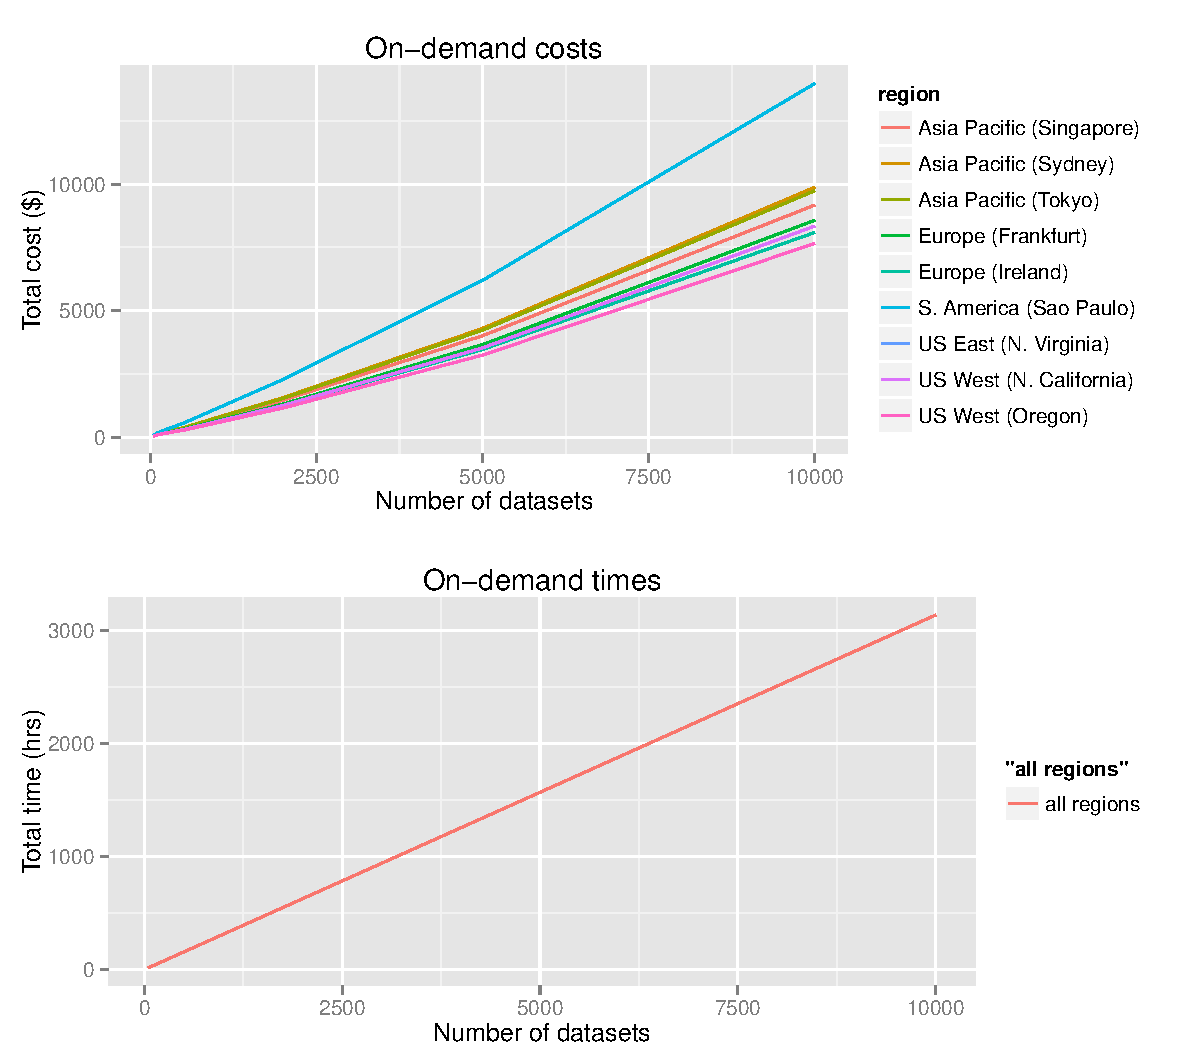
\includegraphics[width=10cm]{../../spot-model/plots/cpac_ondemand.pdf}% This is a *.jpg file
\end{center}
 \textbf{\refstepcounter{figure}\label{fig:01} Figure \arabic{figure}.}{ C-PAC static model costs for on-demand and 1.0x mean spot prices of c3.8xlarge instance }
\end{figure}

%% Results from spot simulations
\subsection{Results from static monte carlo simulations}

The spot model was developed with the same pipeline configuration parameters as the static model except that it used the real history of the per-hour spot price of the c3.8xlarge instance during the processing time in each availability zone. In addition to varying the pipeline, dataset size, and availability zone, this model also varied the per-hour bid-price for running the compute nodes.

The spot model was simulated across all 23 availability zones on AWS, varying dataset sizes from 50 to 10,000 as in the static model; the bid ratio was also varied from 1.0, incrementally up to 5.0 to help develop a bidding strategy based on spot history. The on-demand prices vary between regions, but the spot market prices vary between availability zones (multiple zones per region).

A comparison between the on-demand static model and spot-model is shown in figure \ref{fig:02}, where the mean runtimes and prices are plotted with the on-demand quantity being shown as a black line in each plot. This plot shows that one can typically save much on cost by bidding in the spot market. It can be seen that the lower bound on runtime is always determined by on-demand instances, as they never face forced termination. However, the upper bound on cost is not determined by on-demand instances necessarily; the spot price can sometimes exceed the on-demand price (as is the case with the northern California region plot in purple in figure \ref{fig:02}).

% Spot costs/times
\begin{figure}[!ht]
\begin{center}
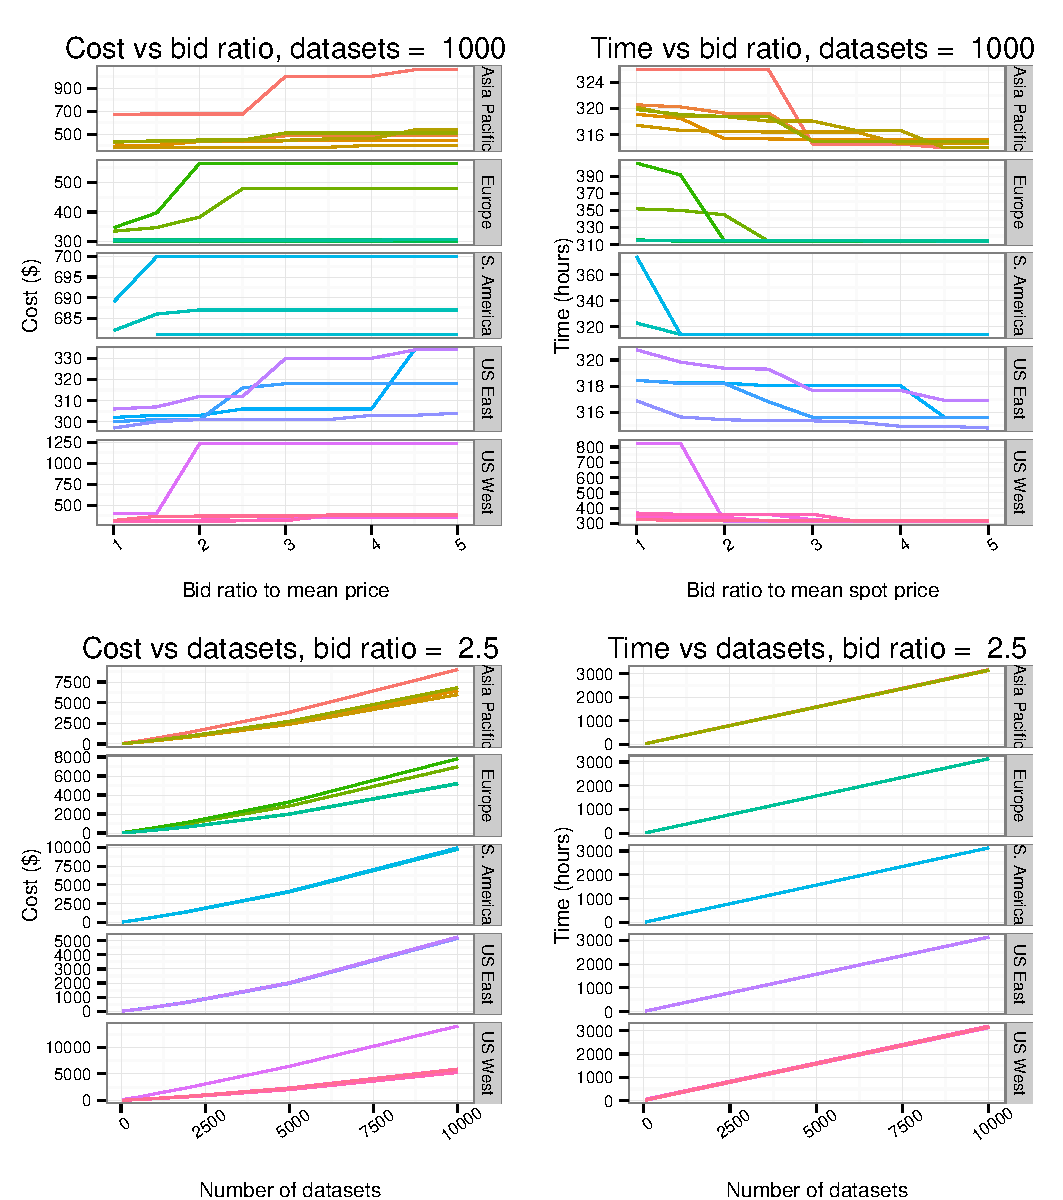
\includegraphics[width=10cm]{../../spot-model/plots/cpac_sim_mean.pdf}% This is a *.jpg file
\end{center}
 \textbf{\refstepcounter{figure}\label{fig:02} Figure \arabic{figure}.}{ C-PAC mean runtimes and costs versus bid ratio; the black lines are the on-demand times and prices }
\end{figure}

It can be seen in figure \ref{fig:02} that the biggest deciding factor for setting a bid ratio to ensure optimal time/cost for one's goal is dependent on availability zone. This is more plainly illustrated in the violin plots of figures \ref{fig:03} and \ref{fig:04}.  However, the cost and runtimes within an avability zone demonstrates a fairly repeatable pattern across pipelines - so it behooves us to focus on the trade-offs of a particular availability zone, or group of availability zones (AWS region). 

Focusing on the US East, northern Virignia, region - it can be seen that the cost for running 1000 datasets really increases after setting a bid ratio of 3.0x. However, a bigger time reduction seems to happen at a bid ratio of around 2.0x; in other words, there is more of a bang for buck at a bid ratio of 2.0x than 3.0x.

\subsubsection{price and time vs. num datasets}
\subsubsection{price and time vs. num nodes}
\subsubsection{price and time vs. instance types}

%% Monte carlo vs static simulations
\subsection{Monte carlo vs static simulations}



% Discussion
\section{Discussion}

\subsection{Comparison of cloud vs. computer ownership}

\subsection{Strategies for spot bidding}

\subsection{Finding optimal computing configurations}

\subsection{Improving performance}

% Conclusions
\section{Conclusions}

Additional Requirements:

\section*{Disclosure/Conflict-of-Interest Statement}
%Frontiers follows the recommendations by the International Committee of Medical Journal Editors (http://www.icmje.org/ethical_4conflicts.html) which require that all financial, commercial or other relationships that might be perceived by the academic community as representing a potential conflict of interest must be disclosed. If no such relationship exists, authors will be asked to declare that the research was conducted in the absence of any commercial or financial relationships that could be construed as a potential conflict of interest. When disclosing the potential conflict of interest, the authors need to address the following points:
%•	Did you or your institution at any time receive payment or services from a third party for any aspect of the submitted work?
%•	Please declare financial relationships with entities that could be perceived to influence, or that give the appearance of potentially influencing, what you wrote in the submitted work.
%•	Please declare patents and copyrights, whether pending, issued, licensed and/or receiving royalties relevant to the work.
%•	Please state other relationships or activities that readers could perceive to have influenced, or that give the appearance of potentially influencing, what you wrote in the submitted work.

The authors declare that the research was conducted in the absence of any commercial or financial relationships that could be construed as a potential conflict of interest.

\section*{Author Contributions}
%When determining authorship the following criteria should be observed:
%•	Substantial contributions to the conception or design of the work; or the acquisition, analysis, or interpretation of data for the work; AND
%•	Drafting the work or revising it critically for important intellectual content; AND
%•	Final approval of the version to be published ; AND
%•	Agreement to be accountable for all aspects of the work in ensuring that questions related to the accuracy or integrity of any part of the work are appropriately investigated and resolved.
%Contributors who meet fewer than all 4 of the above criteria for authorship should not be listed as authors, but they should be acknowledged. (http://www.icmje.org/roles_a.html)

The statement about the authors and contributors can be up to several sentences long, describing the tasks of individual authors referred to by their initials and should be included at the end of the manuscript before the References section.


\section*{Acknowledgments}
Text Text Text Text Text Text  Text Text Text Text Text Text Text Text  Text Text Text Text Text Text Text Text Text  Text Text Text. Text Text Text Text Text Text  Text Text Text Text Text Text Text Text  Text Text Text Text Text Text Text Text Text  Text Text Text. 


\textit{Funding\textcolon} Text Text Text Text Text Text  Text Text.

\section*{Supplemental Data}
Supplementary Material should be uploaded separately on submission, if there are Supplementary Figures, please include the caption in the same file as the figure. LaTeX Supplementary Material templates can be found in the Frontiers LaTeX folder

Text Text Text Text Text Text  Text Text Text Text Text Text Text Text  Text Text Text Text Text Text Text Text Text  Text Text Text.


\bibliographystyle{frontiersinSCNS_ENG_HUMS} % for Science, Engineering and Humanities and Social Sciences articles, for Humanities and Social Sciences articles please include page numbers in the in-text citations
%\bibliographystyle{frontiersinHLTH&FPHY} % for Health and Physics articles
\bibliography{test}

%%% Upload the *bib file along with the *tex file and PDF on submission if the bibliography is not in the main *tex file

\section*{Figures}

%%% Use this if adding the figures directly in the mansucript, if so, please remember to also upload the files when submitting your article
%%% There is no need for adding the file termination, as long as you indicate where the file is saved. In the examples below the files (logo1.jpg and logo2.eps) are in the Frontiers LaTeX folder
%%% If using *.tif files convert them to .jpg or .png


%\begin{figure}
%\begin{center}
%
\includegraphics[width=10cm]{logo2}% This is an *.eps file
%\end{center}
%\textbf{\refstepcounter{figure}\label{fig:02} Figure \arabic{figure}.}{ Enter the caption for your figure here.  Repeat as  necessary for each of your figures }
%\end{figure}

%%% If you don't add the figures in the LaTeX files, please upload them when submitting the article.

%%% Frontiers will add the figures at the end of the provisional pdf automatically %%%

%%% The use of LaTeX coding to draw Diagrams/Figures/Structures should be avoided. They should be external callouts including graphics.

\end{document}
